\documentclass[11pt,a4paper]{article}

% --- язык и шрифты -----------------------------------------------------------
\usepackage{fontspec}
\usepackage[russian]{babel}
\babelfont[russian]{rm}{Liberation Serif}
\babelfont[russian]{sf}{Liberation Sans}
\babelfont[russian]{tt}{Liberation Mono}
\setmainfont{Liberation Serif}
\setsansfont{Liberation Sans}
\setmonofont{Liberation Mono}

\usepackage[a4paper,margin=2.4cm]{geometry}
\usepackage{amsmath,amssymb}
\usepackage{graphicx}
\usepackage{booktabs}
\usepackage{array}
\usepackage{xcolor}
\usepackage{caption}
\usepackage{listings}
\usepackage[hidelinks]{hyperref}

\captionsetup{font=small,labelfont=bf}
\lstset{
  basicstyle=\ttfamily\footnotesize,
  breaklines=true,
  frame=single,
  framesep=4pt,
  columns=fullflexible,
  keepspaces=true,
  showstringspaces=false,
  backgroundcolor=\color{gray!6},
}

% --- числа, которые меняются после финального прогона -----------------------
% (значения подставляются вручную из results/pck_summary.md)
\newcommand{\Ntest}{846}
\newcommand{\PckFull}{0.643}
\newcommand{\PckFullHD}{0.645}
\newcommand{\PckFullSD}{0.630}
\newcommand{\PckTiles}{0.711}
\newcommand{\PckOracle}{0.808}
\newcommand{\PckPose}{0.772}
\newcommand{\PckPoseFull}{0.787}
\newcommand{\DetPose}{94.2}
\newcommand{\DetPoseFull}{94.2}
\newcommand{\LatPose}{380}
\newcommand{\LatPoseFull}{522}

\title{Детекция 21 ключевой точки кисти\\на изображениях и видео в реальном времени}
\author{Курсовой проект\\[2pt] \normalsize (ФИО, группа)}
\date{2026}

\begin{document}
\maketitle

\begin{abstract}
\noindent
Работа решает задачу оценки позы кисти: по изображению или видеокадру найти
21 ключевую точку (запястье и по четыре точки на каждом из пяти пальцев).
В качестве модели используется готовый ансамбль MediaPipe (PoseLandmarker +
HandLandmarker), метрика качества~--- PCK с нормировкой на \(0.7\cdot\)~размер
головы, как в исходной работе CMU Panoptic Hand DB. Предложен двухступенчатый
пайплайн: поза тела даёт запястье, вокруг него строится квадратный ROI,
и уже на увеличенном кропе лендмаркер кисти находит точки. На \Ntest{}
тестовых изображениях пайплайн с ROI даёт PCK@0.2 = \PckPose{} против
\PckFull{} у прямого запуска на полном кадре; вариант с дополнительным проходом
по кадру~--- \PckPoseFull{}. Дополнительно реализованы пост-рендер видео в mp4
и realtime-демо с вебкамеры.
\end{abstract}

\tableofcontents
\newpage

% ============================================================================
\section{Введение}

Оценка позы кисти нужна в жестовых интерфейсах, анализе языка жестов,
реабилитации, управлении роботами и при создании аватаров. В отличие от позы
тела, кисть~--- мелкий объект с сильной самоперекрываемостью: на типичном
кадре её размер составляет единицы процентов площади, а пальцы могут быть
согнуты и частично скрыты. Поэтому качество детекции сильно зависит от того,
в каком масштабе модель видит кисть.

\paragraph{Цель.} Построить и исследовать пайплайн, который находит 21 ключевую
точку кисти на фото и видео, оценить его метрикой PCK и продемонстрировать
работу в реальном времени.

\paragraph{Задачи.}
\begin{enumerate}
  \item подготовить данные и протокол оценки (разбиение, нормировка ошибки);
  \item реализовать инференс MediaPipe и абляции по способу подачи кадра;
  \item измерить PCK и разобрать ошибки по суставам, стороне и размеру кисти;
  \item реализовать пост-рендер видео и realtime-демо, замерить скорость.
\end{enumerate}

\paragraph{Вклад.} Основной результат~--- количественное сравнение четырёх
способов подачи изображения в один и тот же лендмаркер и калибровка
ROI-пайплайна по позе тела. Показывается, что выигрыш даёт не сама модель,
а масштаб, в котором она видит кисть.

% ============================================================================
\section{Данные}

\subsection{Источник и разметка}

Используется \textbf{CMU Panoptic Hand DB}~\cite{simon2017hand}~--- часть
датасета CMU Panoptic~\cite{joo2015panoptic}. Официальный тестовый набор
содержит \Ntest{} изображений; для каждого есть 21 точка в пиксельных
координатах, признак левой/правой руки и \texttt{head\_size}. Тестовые
изображения берутся из версии \textbf{Voxel51/hand-keypoints} (как в задании),
а пиксельные аннотации~--- из официального архива CMU; соответствие
устанавливается по имени файла.

Проверка консистентности: нормированные координаты из \texttt{samples.json}
после умножения на ширину и высоту совпадают с пиксельными координатами CMU
с медианной ошибкой \(0.000\)~px. То есть два источника описывают одну и ту же
разметку, и можно пользоваться любым.

\subsection{Разбиение}

Официальный \texttt{manual\_train} (1912 изображений) делится на train/val
\textbf{по клипам}: кадры одного видео не должны попадать в разные выборки,
иначе оценка завышается за счёт почти одинаковых соседних кадров. Группы имеют
сильно разный размер, поэтому используется жадная раскладка по клипам, а не
стратифицированный сплит. Пересечений клипов с тестом нет ни в train, ни в val.

\begin{table}[h]
  \centering
  \caption{Состав данных. «кисть, \%» --- медианный размер bbox кисти
  относительно большей стороны кадра; \(0.7h\)~--- медианный масштаб для PCK.}
  \label{tab:dataset}
  % автогенерация: python src/make_tables.py
\begin{tabular}{lrrrrrrr}
\toprule
выборка & изображений & клипов & левых & правых & кисть, \% & <10\,\% & $0.7h$, px \\
\midrule
тест & 846 & 220 & 420 & 426 & 8.7 & 62.8\,\% & 98 \\
train & 1409 & 431 & 696 & 713 & 7.6 & 69.2\,\% & 103 \\
val & 503 & 59 & 244 & 259 & 10.2 & 47.7\,\% & 93 \\
\bottomrule
\end{tabular}

\end{table}

\subsection{Статистика}

Кисть действительно мелкая: медиана~--- около \(9\,\%\) большей стороны кадра,
у \(62.8\,\%\) тестовых изображений~--- меньше \(10\,\%\). Разрешения разные
(\(720\times576\), \(1920\times1080\), \(400\times300\) и др.), поэтому один и
тот же относительный размер соответствует разному числу пикселей. Медианный
порог «правильной» точки PCK@0.2 составляет всего \(19.6\)~px. Это и есть
главная сложность задачи: ошибка в 20~px уже считается промахом.

\begin{figure}[h]
  \centering
  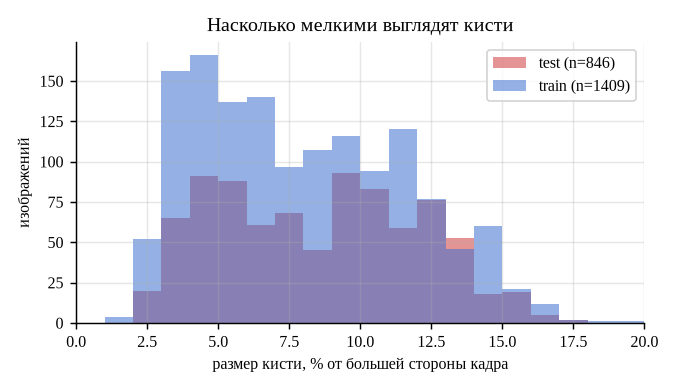
\includegraphics[width=0.78\textwidth]{../results/figs/hand_size_hist.png}
  \caption{Распределение относительного размера кисти в тесте и train.}
  \label{fig:handsize}
\end{figure}

\begin{figure}[h]
  \centering
  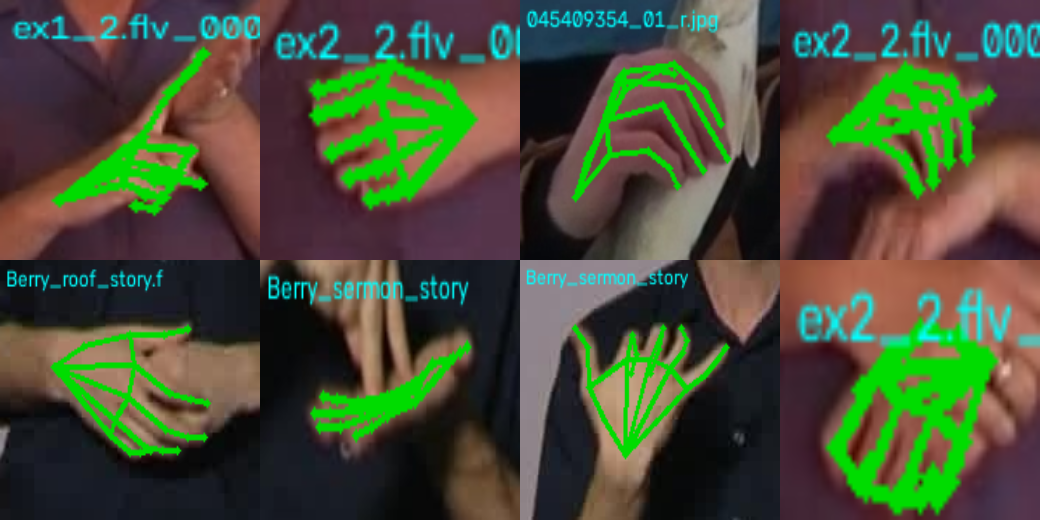
\includegraphics[width=0.86\textwidth]{../results/figs/gt_examples.png}
  \caption{Примеры разметки: зелёным показан GT-скелет в кропе вокруг кисти.}
  \label{fig:gt}
\end{figure}

% ============================================================================
\section{Метрика PCK}

Используется Probability of Correct Keypoint в протоколе авторов датасета.
В работе~\cite{simon2017hand} сказано, что расстояния нормируются на
\(0.7\)~размера головы (примерная длина вытянутой кисти):
\begin{equation}
  \mathrm{PCK}_\alpha
  = \frac{1}{21N}\sum_{i=1}^{N}\sum_{j=1}^{21}
    \mathbb{1}\!\left[\frac{\lVert \hat{\mathbf{p}}_{ij} - \mathbf{p}_{ij}\rVert_2}
                            {0.7\,h_i} \le \alpha\right],
  \label{eq:pck}
\end{equation}
где \(h_i\)~--- \texttt{head\_size} изображения \(i\). Основное число~---
\(\mathrm{PCK}_{0.2}\); дополнительно считаются \(\mathrm{PCK}_{0.1}\), кривая
по \(\alpha\in[0.02,0.5]\) и площадь под ней (AUC).

\paragraph{Пропуск детекции.} Если кисть не найдена, ошибка всех 21 точки
полагается равной \(+\infty\). Альтернатива (исключать такие кадры) завышает
метрику: модель, находящая кисть в половине случаев, выглядела бы не хуже
модели, находящей её всегда.

\paragraph{Выбор предсказания.} В датасете размечена одна рука, а пайплайн
может найти две. Для оценки берётся предсказание с ближайшим к GT запястьем.
Это правило надо учитывать при сравнении: конфигурации, дающие больше
гипотез, получают небольшое преимущество (обсуждается в
разделе~\ref{sec:limits}). Цена показывается колонкой «лишних кистей».

% ============================================================================
\section{Метод}

\subsection{MediaPipe}

MediaPipe Hands~\cite{zhang2020mediapipe}~--- готовый детектор ладони плюс
регрессор 21 точки; порядок точек совпадает с разметкой CMU (запястье, затем
большой, указательный, средний, безымянный и мизинец). Модель обучалась на
кропах вокруг кисти, поэтому критично, какой масштаб ей подать.

В работе используются два бандла:
\begin{itemize}
  \item \texttt{hand\_landmarker.task}~--- 21 точка кисти;
  \item \texttt{pose\_landmarker\_lite.task}~--- поза тела, из неё берутся
        запястья, локти и плечи.
\end{itemize}

\subsection{Двухступенчатый пайплайн}

Обработка кадра:
\begin{enumerate}
  \item кадр приводится к квадрату (letterbox, без искажения пропорций)
        и подаётся в PoseLandmarker;
  \item по плечам и предплечьям оценивается размер кисти
        \(s \approx 0.45\cdot\) (ширина плеч) \(\approx 0.72\cdot\)
        (длина предплечья);
  \item вокруг запястья строится квадратный ROI со стороной
        \(3s\), центр смещается на \(12\,\%\) стороны в сторону пальцев;
  \item кроп масштабируется до \(512\times512\) и подаётся в HandLandmarker;
  \item координаты переводятся обратно в систему исходного кадра.
\end{enumerate}

Квадратность обязательна: при подаче неквадратного ROI MediaPipe выдаёт
предупреждение \texttt{NORM\_RECT without IMAGE\_DIMENSIONS} и возвращает
искажённые координаты. Поэтому и полный кадр, и кроп дополняются до квадрата
чёрными полями, а не растягиваются.

\paragraph{Калибровка.} На 120 случайных тестовых кадрах измерено, что поза
даёт запястье с медианной ошибкой \(0.17\) bbox кисти (p90 \(0.50\)), а
\( \text{bbox} \approx 0.45\cdot\) плечи \(\approx 0.72\cdot\) предплечье.
Свип размера кропа (таблица~\ref{tab:calib}) показал, что тесный кроп
\(\approx 2\times\) bbox теряет кисть, а плато начинается с
\(\approx 3.5\times\) bbox. Для ROI по позе выбран \(3\times\)~bbox:
дальнейшее увеличение кропа уже не помогает, зато повышает шанс, что кисть
окажется у границы из-за ошибки позы.

\begin{table}[h]
  \centering
  \caption{Калибровка размера кропа на 120 кадрах (доля изображений, у которых
  медианная ошибка точки \(\le 0.2\)).}
  \label{tab:calib}
  \begin{tabular}{lcccc}
    \toprule
    кроп & \(1.3\times\) & \(2.2\times\) & \(3.6\times\) & \(4.6\times\) \\
    \midrule
    доля \(\le 0.2\) & 0.508 & 0.725 & 0.808 & 0.825 \\
    детекция & 60.0\,\% & 84.2\,\% & 93.3\,\% & 94.2\,\% \\
    \bottomrule
  \end{tabular}
\end{table}

\paragraph{Страховка и ансамбль.} Если ROI не дал ни одной кисти, выполняется
проход по всему кадру (letterbox в \(960\times960\)). Опционально этот проход
делается всегда (\texttt{ensemble\_full}); результаты склеиваются, если запястья
ближе \(2\,\%\) меньшей стороны кадра (не менее 10~px). Такой радиус убирает
явные дубли, но оставляет альтернативную гипотезу, когда ROI и полный кадр
дают разные оценки.

\paragraph{Сглаживание.} Для видео применяется экспоненциальное сглаживание
точек отдельно для каждой стороны кисти:
\(\hat{\mathbf{p}}_t = \alpha\,\mathbf{p}_t + (1-\alpha)\,\hat{\mathbf{p}}_{t-1}\),
где \(\mathbf{p}_t\)~--- новое предсказание, \(\alpha=0.5\). Оно не меняет
метрику на фотографиях (там режим \texttt{IMAGE} без сглаживания), но убирает
дрожание скелета в демо.

% ============================================================================
\section{Эксперименты}

\subsection{Постановка}

Все конфигурации используют один и тот же лендмаркер и одни и те же веса;
меняется только способ подачи изображения:
\begin{itemize}
  \item \textbf{полный кадр}~--- исходное разрешение, 720p, 480p;
  \item \textbf{2×2 тайла} с перекрытием \(10\,\%\);
  \item \textbf{кроп по GT-bbox} (\(4.6\times\) bbox)~--- верхняя граница
        качества лендмаркера, «оракул»;
  \item \textbf{поза \(\to\) ROI}~--- предлагаемый пайплайн;
  \item \textbf{поза \(\to\) ROI + полный кадр}~--- ансамбль.
\end{itemize}

Замеры выполнены на CPU (4 ядра, без GPU), Python 3.14, MediaPipe 1.2.3.
Задержка~--- время одного вызова на изображение, медиана.

\subsection{Основные результаты}

\begin{table}[h]
  \centering
  \caption{PCK на \Ntest{} тестовых изображениях. Жирным выделен PCK@0.2.}
  \label{tab:pck}
  % автогенерация: python src/make_tables.py
\begin{tabular}{lrrrrrr}
\toprule
конфигурация & PCK@0.1 & PCK@0.2 & AUC & детекция & p50, мс & лишних кистей \\
\midrule
полный кадр & 0.535 & \textbf{0.643} & 0.610 & 83.0\,\% & 152 & 0.60 \\
полный кадр, 720p & 0.540 & \textbf{0.645} & 0.613 & 83.1\,\% & 159 & 0.61 \\
полный кадр, 480p & 0.527 & \textbf{0.630} & 0.598 & 81.4\,\% & 134 & 0.59 \\
2×2 тайла & 0.572 & \textbf{0.711} & 0.677 & 93.3\,\% & 399 & 1.27 \\
поза → ROI (наш) & 0.650 & \textbf{0.772} & 0.728 & 94.2\,\% & 380 & 0.78 \\
поза → ROI + кадр & 0.660 & \textbf{0.787} & 0.743 & 94.2\,\% & 522 & 0.99 \\
кроп по GT-bbox & 0.680 & \textbf{0.808} & 0.765 & 92.0\,\% & 130 & 0.41 \\
\bottomrule
\end{tabular}

\end{table}

\begin{figure}[h]
  \centering
  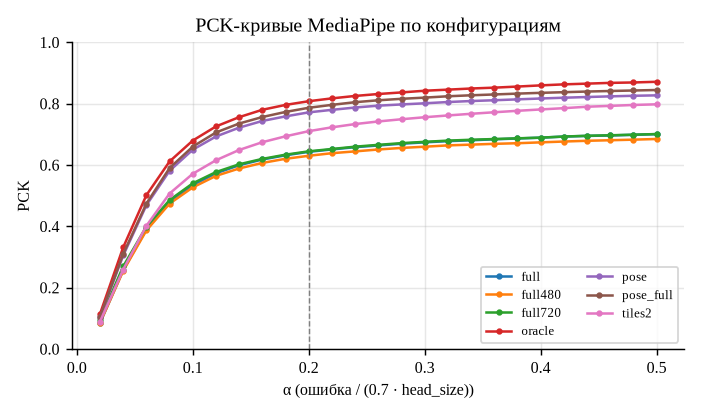
\includegraphics[width=0.64\textwidth]{../results/figs/pck_curve.png}
  \caption{PCK-кривые по \(\alpha\).}
  \label{fig:curve}
\end{figure}

Прямой запуск на полном кадре даёт \(\mathrm{PCK}_{0.2}=\PckFull\), причём
даунскейл до 720p и 480p почти не меняет качество (\(\PckFullHD\) и
\(\PckFullSD\)): модель не столько ошибается в координатах, сколько не находит
мелкую кисть. Кроп по GT-bbox поднимает метрику до \(\PckOracle\)~--- это
показывает, что резерв лендмаркера действительно есть, и он реализуется, если
дать кисть крупно.

Предлагаемый пайплайн с ROI даёт \(\PckPose\): ошибка запястья от позы
(\(\approx 0.17\) bbox) компенсируется запасом кропа \(3\times\). Это
закрывает около \(78\,\%\) разрыва между полным кадром и «оракулом».
Ансамбль с полным кадром даёт \(\PckPoseFull\), но стоит \(+37\,\%\)
задержки и добавляет лишние гипотезы. Тайлы (\(2\times2\)) дают
\(\PckTiles\), однако требуют четырёх вызовов на кадр и находят заметно
больше лишних кистей.

\subsection{Разрезы}

\begin{figure}[h]
  \centering
  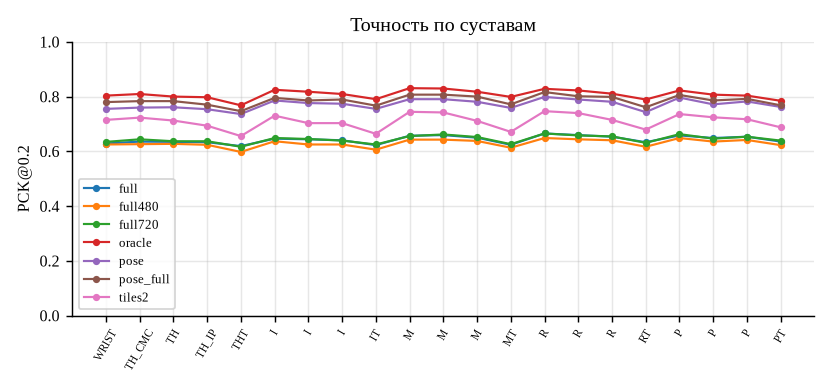
\includegraphics[width=0.80\textwidth]{../results/figs/pck_per_joint.png}
  \caption{PCK@0.2 по суставам: кончики пальцев и большой палец сложнее
  проксимальных суставов.}
  \label{fig:joint}
\end{figure}

\begin{figure}[h]
  \centering
  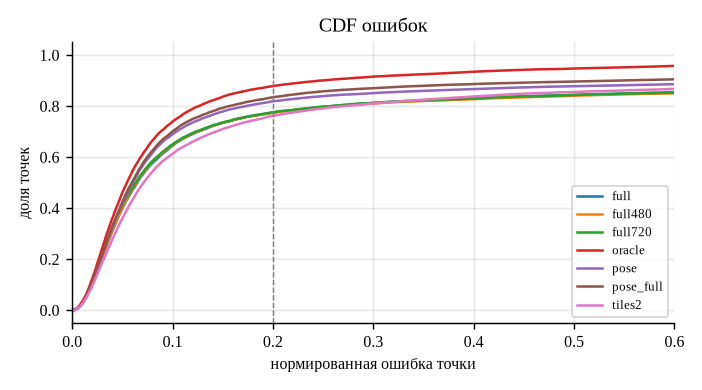
\includegraphics[width=0.62\textwidth]{../results/figs/error_cdf.png}
  \caption{CDF нормированной ошибки точки (по всем найденным точкам).}
  \label{fig:cdf}
\end{figure}

\begin{figure}[h]
  \centering
  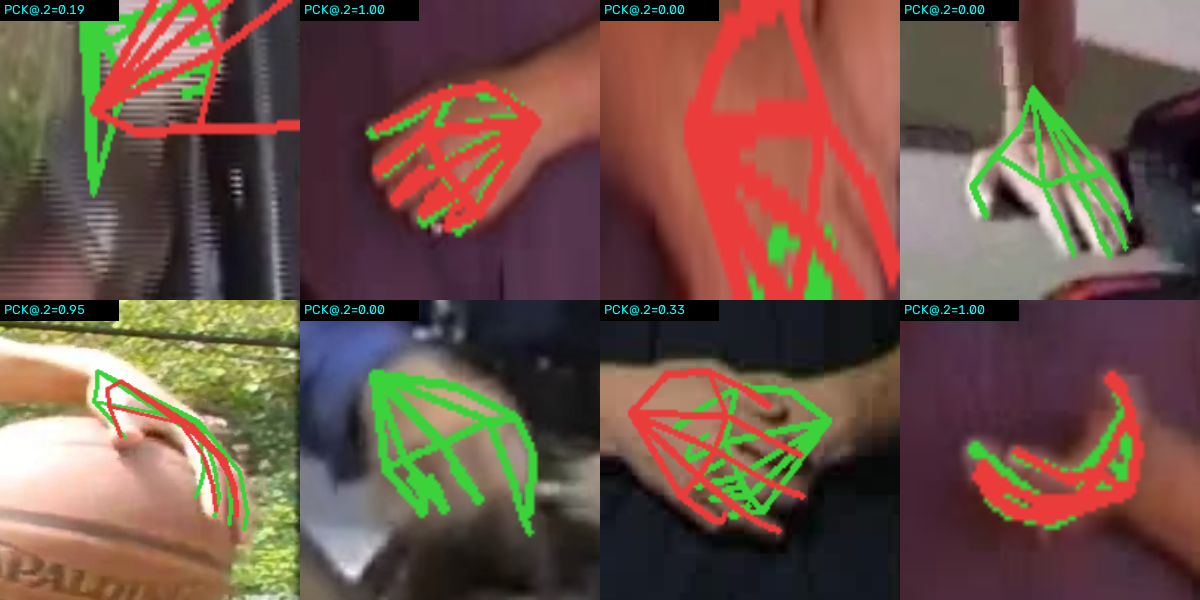
\includegraphics[width=0.82\textwidth]{../results/figs/vis_pose.png}
  \caption{Примеры пайплайна «поза \(\to\) ROI»: зелёный~--- GT, красный~---
  предсказание, в углу~--- PCK@0.2 по кадру. Видны и хорошие совпадения,
  и типичные промахи на мелких/перекрытых кистях.}
  \label{fig:vis}
\end{figure}

\begin{center}
  \captionof{table}{PCK@0.2 в зависимости от размера кисти (доля кадра).}
  \label{tab:size}
  % автогенерация: python src/make_tables.py
\begin{tabular}{lrrr}
\toprule
конфигурация & < 5\,\% & 5–10\,\% & ≥ 10\,\% \\
\midrule
полный кадр & 0.215 & 0.612 & 0.917 \\
полный кадр, 720p & 0.198 & 0.625 & 0.916 \\
полный кадр, 480p & 0.165 & 0.606 & 0.917 \\
2×2 тайла & 0.454 & 0.704 & 0.861 \\
поза → ROI (наш) & 0.532 & 0.757 & 0.922 \\
поза → ROI + кадр & 0.560 & 0.775 & 0.927 \\
кроп по GT-bbox & 0.691 & 0.763 & 0.925 \\
\bottomrule
\end{tabular}

\end{center}

Ожидаемо хуже всего даются самые мелкие кисти (\(<5\,\%\) кадра): полный кадр
там даёт \(\mathrm{PCK}_{0.2}=0.215\), «поза \(\to\) ROI»~--- \(0.532\),
ансамбль~--- \(0.560\), «оракул» по GT-bbox~--- \(0.691\). Именно на мелких
кистях двухступенчатый пайплайн выигрывает в 2,5 раза. Для крупных кистей
(\(\ge 10\,\%\) кадра) все конфигурации почти сравниваются
(\(\approx 0.92\)): модель работает хорошо, когда объект уже крупный, а разница
создаётся условиями съёмки. Кончики пальцев и большой палец ошибаются чаще:
у них больше степеней свободы и сильнее самоперекрытие.

% ============================================================================
\section{Видео и реальное время}
\label{sec:video}

\subsection{Пост-рендер}

Скрипт \texttt{src/infer\_video.py} читает видео, прогоняет кадры через
пайплайн, рисует скелет и HUD (FPS, режим) и пишет H.264 через ffmpeg
(со звуком исходника), с запасным вариантом \texttt{mp4v}. Дополнительно можно
сохранить точки в JSONL для покадрового анализа.

\noindent\begin{minipage}{\linewidth}
\begin{lstlisting}[basicstyle=\ttfamily\scriptsize,breaklines=false,xleftmargin=0pt]
python src/infer_video.py in.mp4 -o out.mp4
python src/infer_video.py in.mp4 --pose-every 3
python src/infer_video.py in.mp4 --no-pose
\end{lstlisting}
\end{minipage}

\subsection{Realtime-демо}

Скрипт \texttt{src/demo\_live.py} открывает вебкамеру и показывает скелет в
окне. Для скорости кадр уменьшается до \(640\times480\), поза пересчитывается
раз в \(N\) кадров (по умолчанию \(N=3\)), ROI~--- \(384\)~px. Клавиши:
\texttt{q}~--- выход, \texttt{s}~--- скриншот, \texttt{p}~--- пауза,
\texttt{f}~--- сглаживание, \texttt{r}~--- запись.

\noindent\begin{minipage}{\linewidth}
\begin{lstlisting}[basicstyle=\ttfamily\scriptsize,breaklines=false,xleftmargin=0pt]
python src/demo_live.py
python src/demo_live.py --fast
python src/demo_live.py --record demo.mp4
\end{lstlisting}
\end{minipage}

На использованной машине без GPU кадр \(640\times360\) обрабатывается за
\(\approx 350\)~мс при пересчёте позы каждый кадр (около \(3\)~FPS); пересчёт
позы раз в 3--5 кадров даёт \(\approx 280\)--\(300\)~мс, потому что основное
время тратит не поза, а два вызова HandLandmarker (по одному на запястье).
Режим «только полный кадр» работает втрое быстрее (\(\approx 110\)~мс,
\(9\)~FPS), но даёт заметно худший PCK. На машине с GPU обе модели
поддерживают аппаратное ускорение, и демо работает плавно; на CPU
интерактивность достигается ценой задержки скелета.

% ============================================================================
\section{Ограничения}
\label{sec:limits}

\begin{itemize}
  \item \textbf{Правило ближайшего запястья.} В датасете размечена одна рука;
        при выборе лучшего из нескольких предсказаний ансамбль получает
        преимущество за счёт дополнительных гипотез. Поэтому основной
        результат~--- конфигурация \texttt{pose}, а ансамбль показан как
        опция с явной ценой (лишние кисти, \(+37\,\%\) задержки).
  \item \textbf{Одна рука в кадре.} Метрика не проверяет вторую руку и
        сценарии с несколькими людьми; для них нужен отдельный протокол
        (например, сопоставление по обеим рукам и штраф за ложные срабатывания).
  \item \textbf{CPU-задержка.} Без GPU интерактивность достигается только
        за счёт уменьшения разрешения и пересчёта позы не каждый кадр.
  \item \textbf{Нормировка на размер головы.} Для изображений без головы
        (сильный кроп, нестандартный ракурс) масштаб PCK не определён; в
        датасете таких нет, но в реальном видео это возможно.
  \item \textbf{Модель не дообучалась.} Использованы готовые веса MediaPipe;
        цель работы~--- исследовать пайплайн и метрику, а не превзойти
        state-of-the-art на CMU.
\end{itemize}

% ============================================================================
\section{Заключение}

Построен и исследован пайплайн детекции 21 ключевой точки кисти на базе
MediaPipe. Показано, что основной прирост даёт не замена модели, а правильный
масштаб: кроп вокруг запястья, построенный по позе тела, поднимает PCK@0.2
с \PckFull{} до \PckPose{}, а кроп по GT-bbox даёт \PckOracle{}, то есть
резерв готового лендмаркера реализуется почти полностью. Реализованы
пост-рендер видео и realtime-демо, замерена скорость на CPU и подобраны
параметры для интерактивного режима.

\paragraph{Воспроизводимость.} Все шаги выполняются скриптами:
\begin{itemize}
  \item \texttt{data/download.py}~--- данные и модели;
  \item \texttt{src/prepare.py}~--- манифест;
  \item \texttt{src/audit.py}~--- аудит данных;
  \item \texttt{src/eval\_mediapipe.py}~--- PCK-эксперименты;
  \item \texttt{src/make\_tables.py}~--- таблицы отчёта.
\end{itemize}
Результаты и графики складываются в \texttt{results/}, отчёт собирается из
\texttt{report/report.tex}.

% ============================================================================
\clearpage
\begin{thebibliography}{9}

\bibitem{simon2017hand}
T.~Simon, H.~Joo, I.~Matthews, Y.~Sheikh.
\newblock Hand Keypoint Detection in Single Images using Multiview Bootstrapping.
\newblock In \emph{CVPR}, 2017.

\bibitem{zhang2020mediapipe}
F.~Zhang, V.~Bazarevsky, A.~Vakunov, A.~Tkachenko, M.~Grundmann, R.~Lempitsky.
\newblock MediaPipe Hands: On-device Real-time Hand Tracking.
\newblock \emph{arXiv:2006.10214}, 2020.

\bibitem{joo2015panoptic}
H.~Joo, H.~Liu, L.~Tan, L.~Guibas, A.~Sheikh.
\newblock Panoptic Studio: A Massively Multiview System for Social Motion Capture.
\newblock In \emph{ICCV}, 2015.

\end{thebibliography}

\end{document}